\begin{figure}[htbp]\centering
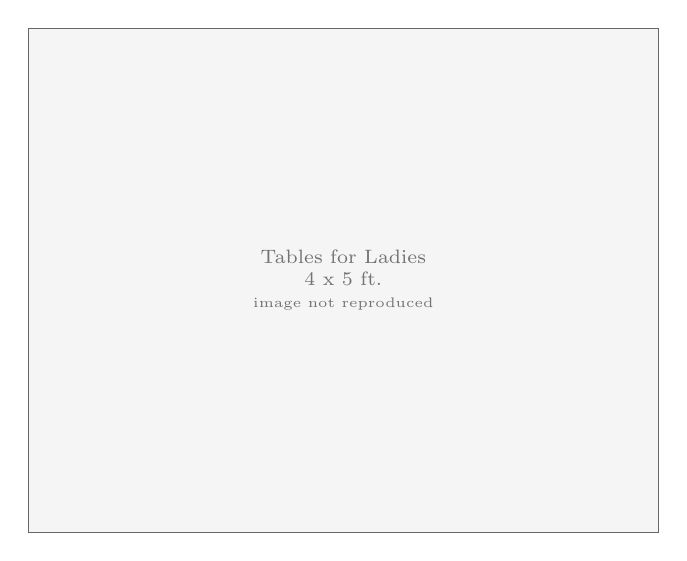
\begin{tikzpicture}
\draw[fill=black!4,draw=black!60,line width=0.5pt] (0,0) rectangle (8,6.4);
\node[align=center,text=black!55,font=\scriptsize] at (4,3.2) {Tables for Ladies\\4 x 5 ft.\\\tiny image not reproduced};
\end{tikzpicture}
\caption{\textbf{Tables for Ladies}, oil, 1930, 4 x 5 ft. as the leaf writes it (Book I, leaf 59, ref 16991). The Metropolitan Museum of Art, Hearn Fund, 1931: \url{https://www.metmuseum.org/art/collection/search/487695}. Scale: sixty inches to eight centimetres. The frames are drawn to the proportions of the size in Edward Hopper's hand; the images are not reproduced here and can be seen at the museums' own pages. Drawn by Claude Fable~5.1, 13 September 2026, from the transcriptions and \texttt{works.json} (2026-09-13).}\label{fig:tables}
\end{figure}
